\documentclass{article} % For LaTeX2e
\usepackage{nips12submit_e,times,soul,amsmath,graphicx,caption,subcaption}
%\documentstyle[nips12submit_09,times,art10]{article} % For LaTeX 2.09


\title{10-725 Final Report -- Fast Point Cloud Registration using Gaussian Processes (TA: Shiva)}


\author{
Ben~Eckart\\
Robotics Institute\\
Carnegie Mellon University\\
Pittsburgh, PA 15213 \\
\texttt{eckart@cmu.edu} \\
\And
Seth Flaxman \\
Machine Learning Department and Heinz College\\
Carnegie Mellon University\\
Pittsburgh, PA 15213 \\
\texttt{sflaxman@cs.cmu.edu} \\
\And
Antonio Juarez \\
Machine Learning Department\\
Carnegie Mellon University\\
Pittsburgh, PA 15213 \\
\texttt{ajuarez@andrew.cmu.edu} \\
}

% The \author macro works with any number of authors. There are two commands
% used to separate the names and addresses of multiple authors: \And and \AND.
%
% Using \And between authors leaves it to \LaTeX{} to determine where to break
% the lines. Using \AND forces a linebreak at that point. So, if \LaTeX{}
% puts 3 of 4 authors names on the first line, and the last on the second
% line, try using \AND instead of \And before the third author name.

\newcommand{\fix}{\marginpar{FIX}}
\newcommand{\new}{\marginpar{NEW}}

\nipsfinalcopy % Uncomment for camera-ready version

\begin{document}


\maketitle

\begin{abstract}

3D range sensing is now ubiquitous in the field of mobile robots. However, many modern 3D range sensors, such as the Velodyne or Kinect, generate massive amounts of data, on the order of one million data points per second,  so it can be challenging to apply standard optimization algorithms for purposes of real-time perception. When given the task of semantic scene understanding, simultaneous localization and mapping (SLAM), tracking, and other low-level perceptual tasks, it is important to be able to reduce these massive point clouds into a more tractable structure to allow real-time computation. We propose transforming the raw data points from 3D sensors to a scene representation based on Gaussian Processes to aid real-time surface construction, registration, and mapping through time. We focus on the registration problem, showing how we can formulate the problem of finding the optimal rigid transformation of a new set of points as an optimization problem. We use {\bf matrix calculus} to derive various solutions to this optimization problem through {\bf backtracking projected gradient descent} and {\bf Newton's method}, and explain how to incorporate extra constraints. Finally, we implement the gradient descent method using {\bf Cholesky decomposition} to insure speed and numerical stability, and compare its performance to the existing Iterative Closest Point (ICP) algorithm.

\end{abstract}

\section{Introduction}

Modeling the environment using maps is one of the cornerstones of mobile autonomy, functioning as an intermediary between raw sensor measurements of the world and high level scene understanding. Spatial maps aid in the tasks of localization, tracking, and object recognition, which in turn are necessary for efficient path planning and higher level perception and intelligence. Parametric or geometric representations of surfaces allow a more compact representation than raw point clouds, which can be massive in scale. These compact representations also allow for standard optimization techniques to be applied to the problem of multiple scan registration, which is a necessary component of any mapping system.

Though sensors such as the Kinect are able to generate massive amounts of data, in many cases this ability is not leveraged and the raw data is modified in such a way that important information is lost. For example, when the environment is roughly rectilinear, such as when the robot is navigating a hallway, nearly all of the points in the cloud can be thought of as coming from a few distinct planes. In this way, we could parametrize our point cloud as a set of planes, not only vastly reducing the space and time complexity of representation, but also the noise inherent in the raw measurements, since plane-fitting uses the most likely estimate \cite{martin_real-time_2002}\cite{liu_using_2001}\cite{thrun_real-time_2004}. However, assuming the world is planar is possibly too limiting of a restriction, especially in environments with clutter or curved surfaces. Past work has used mixtures of Gaussians \cite{tsin2004correlation} \cite{jian2005robust} or Gaussian Processes \cite{plagemann2008nonstationary}, but many of these more expressive formulations come at a higher computational expense and thus cannot be used for real-time perception algorithms.

Assuming a large point cloud can be described parametrically by a few surfaces, new data from the sensor can then be registered to the global frame by associating the points with the known surfaces and optimizing with respect to some measure of fit. Typically, this is done using the Iterative Closest Point (ICP) algorithm, which is a somewhat \emph{ad hoc} greedy algorithm that iteratively refines the associations of points from a reference scan and points from a new scan \cite{besl_method_1992}. By contrast, our proposed formulation has nice properties, and it can be efficiently optimized as we show.

%This surface representation is then fed into a parallel gradient based algorithm to find the best fit between two successive point cloud scans to solve the registration problem.

\section{Proposed Method}

We propose a novel Gaussian Process (GP)-based formulation of the point cloud registration problem.
We state the problem as follows: given a set of 3D points $\mathbf{X}$ ({\bf the scene}), and a set of points $\mathbf{X'}$ ({\bf the new}), find the most likely rigid transformation $T$ of $\mathbf{X'}$ to match the points in $X$. 
To formulate this as an optimization problem, we first use GPs to fit a smooth surface $S$ to $\mathbf{X}$. Then we optimize over
rigid transformations $T$ to maximize the likelihood of seeing transformed points $T(\mathbf{X'})$ given $S$. We parameterize $T$ as a translation in 3D: $(T_x, T_y, T_z)$ and a quaternion rotation in 3D: $T_q = (T_s, T_u, T_v, T_w)$ . Our GP formulation and derivation is in Section \ref{sec:math}.

We propose to use gradient descent and Newton's method to solve our novel registration problem. The formulation and derivations we given in Sections \ref{sec:gradient} and \ref{sec:newton} are original.

 %we can look at the probability of a ``scene'' having generated those points according to some surface model. If the probability of a point is %$p(\mathbf{x_i}|\mathbf{\Theta{}})$, where $\mathbf{\Theta{}}$ is the set of parameters describing the scene, then the total probability of an entire %scan of data is $p(\mathbf{X}|\mathbf{\Theta{}}) = \prod_{i} p(\mathbf{x_i}|\mathbf{\Theta{}})$. In our problem, we wish to optimize over some spatial %transformation in 3D space. Thus, we can minimize over the negative log-likelihood of the data with respect to the transformation parameters,

%$$
%\min_{\mathbf{q},\mathbf{t}} -\log p(T(\mathbf{X}|\mathbf{q},\mathbf{t})|\mathbf{\Theta{}}) = - \sum_i \log  p(T(\mathbf{x_i}|\mathbf{q},\mathbf{t}) | %\mathbf{\Theta{}}) \\
%$$

%where $\mathbf{q}$ and $\mathbf{t}$ are the spatial transformation parameters representing quaternion rotation and translation, respectively. Because the particular problem of point cloud data involves a vast amount of points, we can parallelize the computation of the gradient by computing as much of the gradient as possible independently with CUDA threads and then doing a logarithmic number of reductions to obtain the final gradient step. Minimizing over the above equation will provide the maximum likelihood spatial transformation of the data to the scene, and will allow us to register together successive 3D measurements and recover the motion of the sensor.

%\section{Previous Work and Milestones}
%One of the group members (Ben) has done previous work in this area, coming up with a parallel Expectation Maximization algorithm for point cloud segmentation into a Gaussian mixture model (GMM). We believe that a Gaussian Process formulation, however, would provide more flexibility while providing some of the same computational benefits as a GMM formulation. 

%The work can be divided into two separate, but related, optimization problems: The first problem is to transform a point cloud using Gaussian Processes so that the spatial representation of surfaces can be continuous. The second problem involves taking such a representation and finding the most likely rigid spatial transformation given a new set of range data representing the same scene. When the rigid spatial transformation is found, the scene and new data can then be fused together. If done in real-time, this process can be iterated as a continuous registration loop in a mapping system for a moving robot.

%As our first milestone we will demonstrate feasibility by writing a serial version of our two optimization problems to operate in a simulated 2D environment. For our second milestone, we will build a parallel CUDA version, and extend it to the 3D case. Finally, this algorithm will then be applied to pre-recorded Kinect data. If the speed of the proposed methods is sufficient for real-time computation, the methods outlined here could then be applied to a moving robot with onboard Kinect sensing. These milestones could be completed in a perfect world, but we will consider our project to be successful if we can develop and implement a parallel surface construction and registration algorithm and run it on simulated 3D data, even if it isn't necessarily in real-time or on real-world (noisy, occluded) data. 

%After a discussion with Shiva, we revised our first milestone to be that of understanding the theory underlying our problem and formalizing our objective as an optimization problem. In the next two sections we present related work and our optimization problem.

\section{Related Work}

Point cloud registration algorithms have appeared in many fields, including computer graphics, medical imaging, surveying, reverse engineering, and robotics. As our application concerns real-time perception for robots, we will focus on those techniques that sacrifice exact estimation for real-time speeds. 

Two broad categories of point cloud registration algorithms exist: those that do direct point-to-point or point-to-local-surface matching, and those that first parametrically transform one or both point clouds into a new object with better computational properties before calculating the rigid transformation. The former catgory includes the widely used Iterative Closest Point (ICP) algorithm, and the latter includes registration algorithms based on planar segmentation, Gaussian Mixture Models (GMM), or Normal Distance Transforms (NDT). 

\subsection{ICP}

First developed by Besl and McKay~\cite{besl_method_1992}, ICP works to iteratively associate points between two point clouds and to minimize the squared error between the associated points under rigid transformation parameters. The basic steps are as follows:

\begin{enumerate}
 \item Sample points from each cloud (or use entire cloud)
 \item For each point in a given cloud, find a corresponding point (e.g. via Euclidean distance)
 \item Assign weights to the correspondences
 \item Reject outlier pairs
 \item Apply an error metric to the current transform (e.g. sum of squared error)
 \item Use an optimization technique to minimize the error metric (e.g. SVD, gradient descent, Newton's method, etc.)
\end{enumerate}

ICP is somewhat ill-posed given the fact that each point cloud consists of non-uniform point samples and thus a given point is very unlikely to have an exact corresponding point in the other point cloud. Furthermore, if outliers are not properly caught and discarded, then trying to minimize outliers using the squared distance will not be robust and can cause the algorithm to diverge. 

Many variants of ICP have been proposed and used with varying degrees of success~\cite{mitra_registration_2004}. Typically, the modifications center around avoiding the computational expense of having to find nearest neighbors for every point. Some effective advancements toward this goal include the use of Octrees for approximate nearest neighbor calculations or fast projections~\cite{rusinkiewicz2001efficient}. 

\subsection{Surface Models}

Many registration algorithms first begin with an explicit or implicit parameterization of the point cloud into a form that provides continuous point estimates. Many of the fastest parameterizations are in the form of planar models. The task of point cloud registration then reduces to a problem over finding the best transformation of a set of planes\cite{martin_real-time_2002}\cite{liu_using_2001}\cite{thrun_real-time_2004}. Given a set of new points, the corresponding point in the scene can simply be the closest surface in terms of point-to-plane distance. In this way, the matching process has better convergence properties than ICP, since the matching is from points to corresponding surfaces and not simply to other sampled points. Furthermore, since many indoor environments are roughly rectilinear, the planar decomposition of the environment given a point cloud is somewhat justified. 

Other techniques use distance transforms or Gaussian Mixture Models to describe the point cloud\cite{tsin2004correlation} \cite{jian2005robust}. Normal Distance Transform methods discretize the point cloud into cubic regions (voxels) and compute Gaussian distribution parameters for each voxel \cite{biber2003normal}. Given that each voxel now contains a probabilistic interpretation of a point falling into it, the likelihood has a well-defined gradient and the optimization over the rigid transformation can be more robust than a method like ICP.

\subsection{Comparison to Related Work}

We are developing a parametric surface model under the Gaussian Process framework. Since we do not have to find a nearest neighbor for every point, as is the case in ICP, the optimization can be reduced to efficient inversion of the covariance matrices that appear in the calculations in Section \ref{sec:math}. Furthermore, this formulation allows us to specify gradients with respect to a likelihood under the rigid transformation parameters. For ICP, the metric is simply sum of squared error, which has no such probabilistic foundation. Our work is closely related to surface models, though we choose to let the environment be composed of non-planar regions, giving more flexibility to our model than the planar environment models. Finally, we do not have the discretization problems of the NDT, and we do not need to use a clustering algorithm such as EM as a preprocessing step to find the GMM parameters for the point cloud. 


\section{Theoretical Development}
\label{sec:math}

\subsection{Gaussian Processes}
Gaussian Processes provide an attractive formalism for modeling spatial data. Described in detail in \cite{rasmussen2006gaussian}, we make use of
them in the regression context, fitting a smooth distribution of surfaces to point data in 3-dimensions. Given a new set of point data, our registration problem becomes an optimization problem: find the best rigid transformation of the new data to match the already calculated distribution of surfaces. Below we describe our optimization problem in terms of
maximizing the log-likelihood of a Gaussian distribution, using the key feature of Gaussian Processes, that when making predictions at
a finite set of locations, the Gaussian Process becomes a multivariate Gaussian distribution. Important practical considerations not discussed below include choosing and tuning a suitable kernel, and computational challenges in quickly computing the inverse of the various large matrices described below.

\subsection{Rigid Transformations with Quaternions}
Given a point $x = (x_1,x_2,x_3)^T$ in $\mathcal{R}^3$, we will define a rigid transformation (rotation and translation) as:
$$T(x) := q [x_1, x_2, x_3, 0]^T \bar q +t = R(q) x + t$$ where $q = (s,u,v,w)$ is a unit quaternion, $R$ is the $3 \times 3$ rotation matrix uniquely defined by $q$ (see \cite{wheeler1995}, page 3),

\begin{equation}
R(q) := \left[ \begin{array}{ccc}
s^2+u^2-v^2-w^2 & 2(uv-sw) & 2(uw+sv)\\
2(uv+sw) & s^2-u^2+v^2-w^2 & 2(vw-su)\\
2(uw-sv) & 2(vw+su) & s^2-u^2-v^2+w^2\end{array} \right].
\end{equation} 

and $t \in \mathcal{R}^3$ is a translation vector. We will work in terms of quaternions because this will yield a simple form for the gradient of $T$. 


%Define $C(x)$ to be the skew-symmetric matrix of $x$:
%
%$$C(x) := \left[ \begin{array}{ccc}
%0 & -x_3 & x_2 \\
%x_3 & 0 & -x_1 \\
%-x_2 & x_1 & 0 \end{array} \right].$$
%
%Then, following \cite{wheeler1995}, the gradient of $T$ can be derived with respect to the unit quaternion $q$ and translation $t$:
%$$\frac{\partial T}{\partial q}= 2C(R(q)x)^T$$
%$$\frac{\partial T}{\partial t}= 1$$

\subsection{Formulating an Optimization Problem}
Towards our ultimate goal of describing any rigid set of points in three dimensions, we treat a set of 3D points as elevation data, where given a set of $N_1$ points $\mathbf{X} = \{(x_i,y_i,z_i)^{T}\}$, we interpret $(x_i,y_i)$ as locations in a plane, and $z_i$ as the elevation above the plane. We use Gaussian Processes to fit the scene $\mathbf{X}$, learning a distribution over functions $f(x,y) = z$ which we denote as $f \sim \mbox{GP}(m,K)$. Given the new scene $\mathbf{X'} = \{(x'_i,y'_i,z'_i)^{T}\}$ comprised of $N_2$ points, our objective is as follows: learn a rigid transformation $T$ that maximizes the probability that the points $T(\mathbf{X'})$ were drawn from the same distribution $\mbox{GP}(m,K)$. Conceptually, we are learning a distribution over surfaces given $\mathbf{X}$ and then looking for a rigid transformation $T$ of $\mathbf{X'}$ for which the transformed points are likely to have been generated by the distribution.

Given the scene $\mathbf{X} = \{(x_i,y_i,z_i)^T\}$ and a set of locations $\mathbf{X}_{*} = \{(x_{i*},y_{i*},z_{i*})^T\}$ in the scene, we can write the predictive equations for Gaussian process regression, following \cite{rasmussen2006gaussian}:
\begin{eqnarray}
z_{*} | \mathbf{X}, x_*,y_* &\sim& \mathcal{N}(\mu_*, \Sigma_*) \\
\mu_* &=& K_*[K + \sigma_n^2 I]^{-1} z \\
\Sigma_* &=& K_{**} - K_*[K + \sigma_n^2 I]^{-1} K_*^T
\end{eqnarray}

%This is a multivariate Gaussian distribution, so its likelihood is (\hl{what is D?}):
%$$\mathbf{L}(z_*|\mathbf{X}, x_*,y_*) = (2\pi)^{-D/2} |\Sigma_*|^{-1/2} \exp(-\frac{1}{2} (z_* - \mu_*)^T \Sigma^{-1} (z_* - \mu_*))$$

Here, $K$, $K_*$, and $K_{**}$ denote the Gram matrices $K(\mathbf{X},\mathbf{X})$, $K(\mathbf{X}$,$\mathbf{X_*}$), and $K(\mathbf{X_*},\mathbf{X_*})$, respectively. If we are given the new points $\mathbf{X'}$ and we want to register them to $\mathbf{X}$ then we need to find a rigid transformation $T$. We define $\mathbf{X_*} = T(\mathbf{X'}) = R(q)\mathbf{X'} + t$, where $q = (T_s, T_u,T_v,T_w)$ and $t = (T_x, T_y, T_z)$. 


Thus, our optimization problem is to maximize the likelihood of the multivariate Gaussian distribution over transformations $T$:
\begin{equation}
\max_T \mathcal{L}(T|\mathbf{X}, \mathbf{X'}) = (2\pi)^{-D/2} |\Sigma_*|^{-1/2} \exp(-\frac{1}{2} (z_* - \mu_*)^T \Sigma_*^{-1} (z_* - \mu_*))
\end{equation}

%where we similarly substitute:
%\begin{eqnarray}
%z_* | X, y, T(X') &\sim& \mathcal{N}(\mu_*, \Sigma_*) \\
%\mu_* &=& \mathbf{E}[z_* | X,y,T(X')] = K_*[K + \sigma_n^2 I]^{-1} y \\
%\Sigma_* &=& K_{**} - K_*[K + \sigma_n^2 I]^{-1} K_*^T
%\end{eqnarray}

\subsection{Gradient Descent}
\label{sec:gradient}
Our first solution to  this optimization problem is by gradient descent. 
We calculate the gradient of the log-likelihood by taking partial derivatives with respect to the rotation $q = (T_s, T_u,T_v,T_w)$ and the translation $(T_x, T_y, T_z)$, using the derivations from the previous section:

\begin{equation}
\log \mathbf{L} = -\frac{D}{2} \log (2\pi) - \frac{1}{2} \log \det \Sigma_* - \frac{1}{2} \left((z_* - \mu_*)^T \Sigma_*^{-1} (z_* - \mu_*)\right)
\end{equation}
\begin{eqnarray}
\frac{\partial \log \mathbf{L}}{\partial q} &= - \frac{1}{2} \mbox{tr}(\Sigma_*^{-1} \frac{\partial}{\partial q} \Sigma_*)
                - \frac{\partial}{\partial q} \frac{1}{2} \left((z_* - \mu_*)^T \Sigma_*^{-1} (z_* - \mu_*)\right) 
\label{eq-partialq}
\end{eqnarray}

First, we derive the partial of $\Sigma_*$ with respect to $q$:

\begin{eqnarray}
\frac{\partial}{\partial q} \Sigma_* &=& \frac{\partial}{\partial q} (K_{**} - K_*[K + \sigma_n^2 I]^{-1} K_*^T) \nonumber\\
&=& \frac{\partial K_{**}}{\partial q} + \frac{\partial}{\partial q} (- K_*[K + \sigma_n^2 I]^{-1} K_*^T) \nonumber\\
&=& \frac{\partial K_{**}}{\partial q} - \frac{\partial K_*}{\partial q}  \left[K + \sigma_n^2 I\right]^{-1} K_*^T \nonumber\\
&&  - ~ K_* [K + \sigma_n^2 I]^{-1} \frac{\partial K_*^T}{\partial q}  \label{eq-covpartialq}
%&=& \mbox{\hl{???}} -( A B C + C^T B^T A^T)\\
%&=& \mbox{\hl{???}} -( A B C + (A B C)^T)\\
%&=& \mbox{\hl{???}} -( X + X^T)\\
%&=& -L(T(X'),X) [K + \sigma_n^2 I]^{-1} K_*^T \\ 
%&& (K_*) [K + \sigma_n^2 I]^{-1} L(X,T(X'))
\end{eqnarray}
 
%Our computation will be aided by noting that this expression has the form $A + A^T$ for some matrix $A$.

 We can derive the matrix $\frac{\partial}{\partial q} K_*$ as follows where the $(i,j)$th entry of $K_*$ is given by $k(\mathbf{x}_{i*}, \mathbf{x}_j)$ for a kernel $k$:
\begin{eqnarray}
\left(\frac{\partial K_*}{\partial q}\right)_{ij} = \frac{\partial}{\partial q} k(\mathbf{x}_{i*}, \mathbf{x}_j) = k'(\mathbf{x}_{i*}, \mathbf{x}_j)^T \frac{\partial \mathbf{x}_{i*}}{\partial q}  = k'(\mathbf{x}_{i*}, \mathbf{x}_j)^T \frac{\partial}{\partial q} R_{12}(q)\mathbf{x}'_i
\label{equation:partialKq}
\end{eqnarray}
In the above equation the bolded $\mathbf{x}_j$ refers to the first two components of the $j$th element of $\mathbf{X}$ (likewise for $\mathbf{x_*}$ and $\mathbf{x'}$). Additionally, $R_{12}(q)$ refers to the first two rows of the rotation matrix formed by $q$. The partial derivative of the kernel function depends on our choice of kernel. For this paper, we chose to use the squared exponential kernel, defined as:

\begin{equation}
k(x_i,x_j) = k_1\exp(-0.5*k_2||x_i-x_j||^2)
\end{equation}

Setting the parameters $k_1 = k_2 = 1$, our final equation for the partial of $K_*$ is:

\begin{eqnarray}
\left(\frac{\partial K_*}{\partial q}\right)_{ij} = -(\mathbf{x}_{i*} - \mathbf{x}_j)^T k(\mathbf{x}_{i*}, \mathbf{x}_j) \frac{ \partial R_{12}(q)}{\partial q} \mathbf{x}'_i
\label{equation:partialKqFinal}
\end{eqnarray}

The partial of $K_{**}$ using the squared exponential kernel takes on a similar form, except both vectors in the kernel arguments have a nonzero partial derivative with respect to $q$:

\begin{eqnarray}
\left(\frac{\partial K_{**}}{\partial q}\right)_{ij} = -(\mathbf{x}_{i*} - \mathbf{x}_{j*})^T k(\mathbf{x}_{i*}, \mathbf{x}_{j*}) \frac{ \partial R_{12}(q)}{\partial q} (\mathbf{x}'_i - \mathbf{x}'_j)
\label{equation:partialKstarstarqFinal}
\end{eqnarray}

For the second term in Equation \ref{eq-partialq} we apply the product rule and thus need to evaluate two partial derivatives:

\begin{equation}
\frac{\partial}{\partial q} (z_* - \mu_*) = \frac{\partial}{\partial q} z_* - \frac{\partial}{\partial q} \mu_*
=  \frac{\partial R_3(q)}{\partial q}z' - \frac{\partial}{\partial q} (K_*[K + \sigma_n^2 I]^{-1} z)$$
$$= \frac{\partial R_3(q)}{\partial q}z' - \frac{\partial K_*}{\partial q} \left[K + \sigma_n^2 I\right]^{-1} z
\end{equation}

Here $R_3$ denotes the third row of $R$. Note that the partial of $K_*$ was previously derived in Equation~\ref{equation:partialKqFinal}.

Dealing with the middle term of the second term in Equation \ref{eq-partialq} requires evaluating this partial derivative:
\begin{eqnarray}
\frac{\partial}{\partial q} \left(\Sigma_*^{-1}\right) = -\Sigma_*^{-1} \frac{\partial}{\partial q}\left(\Sigma_*\right) \Sigma_*^{-1}
\label{eq:inversecov}
\end{eqnarray}

where we used the identity $\partial(X^{-1}) = - X^{-1} (\partial X) X^{-1}$ \cite{petersen2008matrix}. We already derived $\frac{\partial}{\partial q} (\Sigma_*)$ above in Equation \ref{eq-covpartialq}.

For space, we do not show the final expression. We also need to find $\frac{\partial \log \mathbf{L}}{\partial t}$. This is essentially
equivalent to the preceding derivation, with the following simplification: $\frac{\partial }{\partial t} T(x'_i) = 1$.

To implement gradient descent, we use the gradient in our update step. We used the standard backtracking line search to find a suitable step-size. Backtracking line search iteratively descreases the stepsize while evaluating the likelihood function to find a suitable descent amount \cite[p. 464]{boyd2004convex}.

\subsection{Projected gradient descent}
As explained in \cite{wheeler1995}, although quaternions have 4 parameters, the space of rotations in 3D is best parameterized by quaternions of length 1. This turns our unconstrained optimization problem into a constrained problem with a simple constraint: $||T_q||^2_2 = 1$. We can solve this problem using projected gradient descent: after doing the gradient update, we simply project the new parameter $T$ to the space in which $||T_q||^2_2 = 1$
by renormalizing: $T_q' = \frac{T_q}{||T_q||^2_2}$.

In Figure \ref{figure:likelihood} in the Appendix, we show a likelihood surface based on synthetic data, projected into 3D. Notice that globally, the problem is not convex, but that there is a well-behaved bowl-shaped region near the origin. Practically, we know that two scenes that we are trying to register will represent pictures of the world taken very close in time (i.e.~1/30th of a second), and thus the rotation and translation will not be large because the sensor will be moving smoothly and slowly compared to the frame rate. Thus, it makes sense to consider further constraining our optimization problem to small translations and rotations. For translations, the simplest way to do this is to constrain the length of the translation vector: $\|T_x^2 + T_y^2 + T_z^2\|^2_2 \leq \epsilon_1$. For rotations, a small rotation angle is equivalent to having the real component of the quaternion, $T_s$, be close to $1$ \cite{wheeler1995} (the intuition is that for a unit length quaternion $T_q$, if $T_s$ parameter is close to $1$, $T_q$ is close to the identity quaternion $[1, 0, 0, 0]^T$). Thus we add the constraint $T_s^2 \geq 1-\epsilon_2$.

We can again use projected gradient descent to incorporate these two new constraints: for each gradient update step we first normalize $q$ as described above, then we check whether $\|T_x^2 + T_y^2 + T_z^2\|^2_2 \leq \epsilon_1$ and if not, we linearly scale it so that $\|T_x^2 + T_y^2 + T_z^2\|^2_2 = \epsilon_1$. Finally, we check whether $T_s^2 \geq 1-\epsilon_2$. If not, we set $T_s^2 = 1-\epsilon_2$ and renormalize $T_q$ to be a unit-length quaternion. 

\subsection{Newton's method}
\label{sec:newton}
Once we've done the work of calculating the gradient, the derivation of the Hessian is a natural, albeit quite math-intensive, extension. Newton's method requires inverting the Hessian, which is a $7 \times 7$ matrix, so this is a relatively cheap operation, and we expect that Newton's method will show large improvements in terms of the convergence rate as compared to gradient descent. We show parts of the derivation, omitting full details for space\footnote{We further note that it is possible to numerically approximate the Hessian from the analytically derived gradient. In practice, this approach may give suitable results while avoiding implementation errors.}:
\begin{align*}
\frac{\partial^2 }{\partial T_x \partial T_y} \Sigma &= \frac{\partial^2}{\partial T_x \partial T_y} K_{**} - \left(\frac{\partial^2}{\partial T_x \partial T_y}K_{*}\right) [K + \sigma^2 I]^{-1} K_*^T - K_{*} [K + \sigma^2 I]^{-1} \left(\frac{\partial^2}{\partial T_x \partial T_y} K_*^T\right) \\
\end{align*}
The first term is 0, and the others depend on the choice of kernel as in the previous section. Derivations with $T_z$ and $T_q$ are similar.

The second term in the likelihood requires finding:
\begin{align*}
\frac{\partial^2 }{\partial T_x \partial T_y} (z_* - \mu_*) &= \frac{\partial^2 }{\partial T_x \partial T_y} (- \mu_*) 
= \frac{\partial^2 }{\partial T_x \partial T_y}( K_* [K+\sigma^2 I]^{-1} z)
= (\frac{\partial^2 }{\partial T_x \partial T_y} K_*) [K+\sigma^2 I]^{-1} z
\end{align*}
Again, this depends on the choice of kernel. Derivations with $T_z$ and $T_q$ are similar, requiring the correct application of matrix calculus as in the previous section. To finish the derivation, we proceed as in the previous section. Taking another partial derivative of Equation \ref{eq:inversecov} is quite messy, requiring repeated application of the product rule and the identity  $\partial(X^{-1}) = - X^{-1} (\partial X) X^{-1}$.

%\begin{figure}[h]
%\begin{center}
%%\framebox[4.0in]{$\;$}
%\fbox{\rule[-.5cm]{0cm}{4cm} \rule[-.5cm]{4cm}{0cm}}
%\end{center}
%\caption{Sample figure caption.}
%\end{figure}

 
\begin{figure}
        \centering
        \begin{subfigure}[b]{0.5\textwidth}
                \centering
                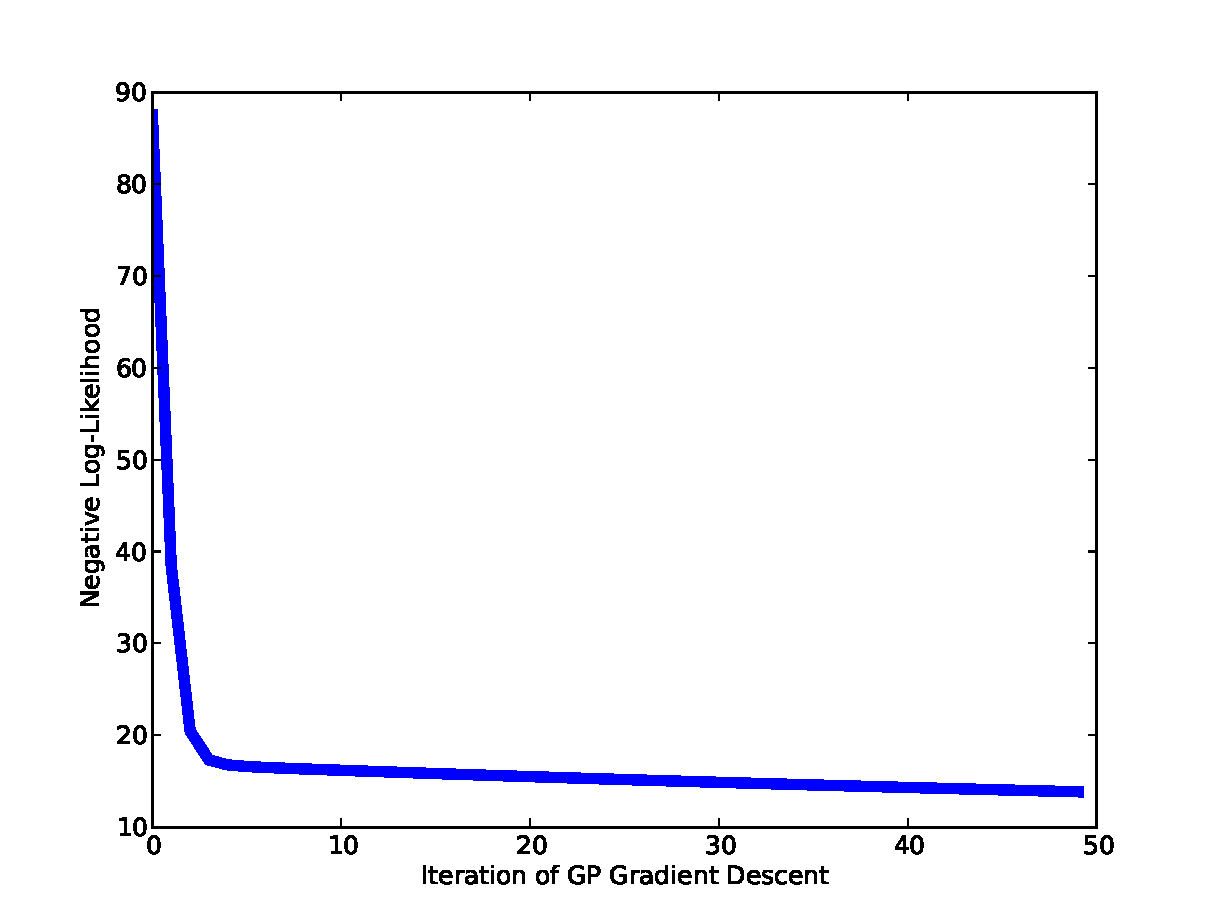
\includegraphics[width=\textwidth]{LL.pdf}
                \caption{Convergence rate }
                \label{fig:elevation}
        \end{subfigure}%
        ~ %add desired spacing between images, e. g. ~, \quad, \qquad etc. 
          %(or a blank line to force the subfigure onto a new line)
        \begin{subfigure}[b]{0.5\textwidth}
                \centering
                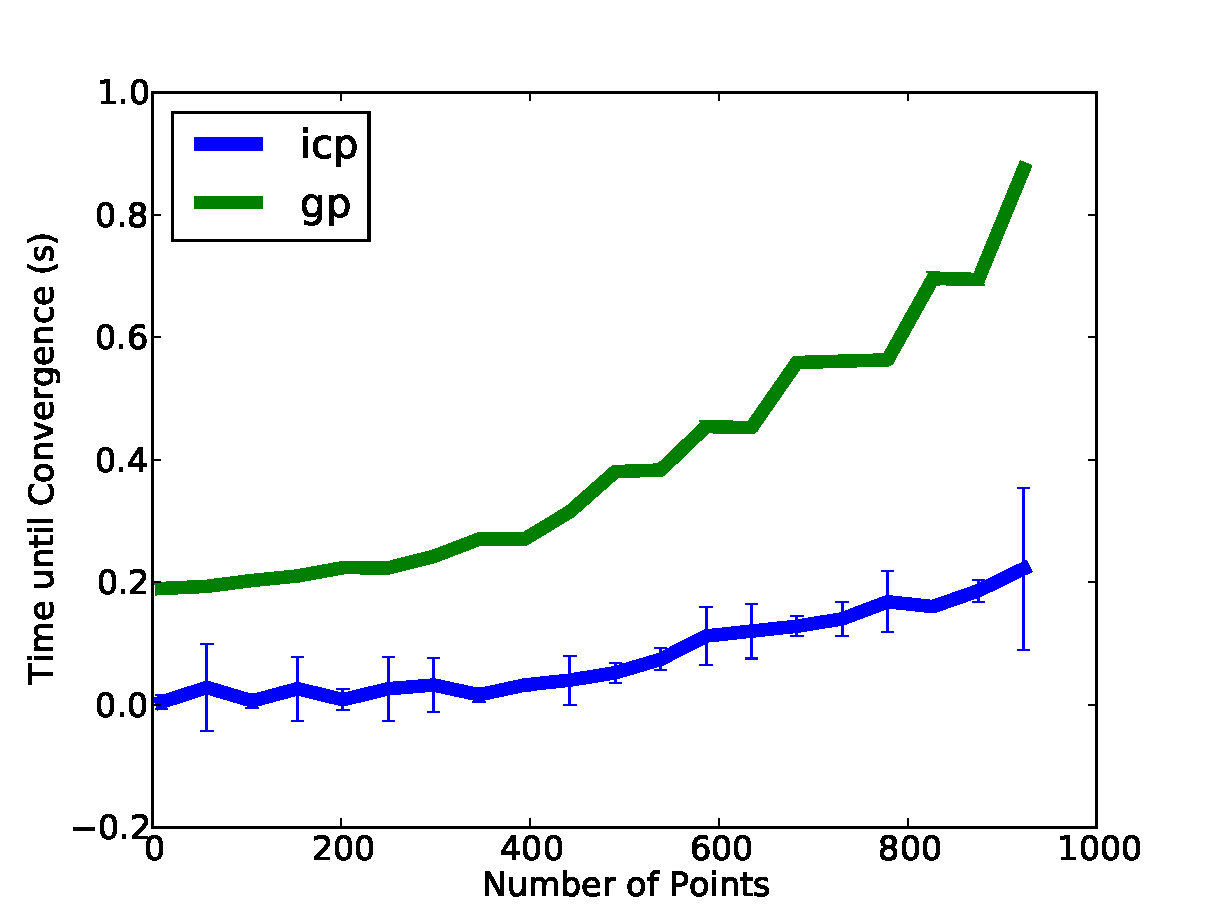
\includegraphics[width=\textwidth]{scaling3.pdf}
                \caption{Time until convergence for different $N_1$}
                \label{fig:mean}
        \end{subfigure}
        \caption{Summary here...}\label{fig:GP}
\end{figure}

\begin{figure}
        \centering
        \begin{subfigure}[b]{0.5\textwidth}
                \centering
                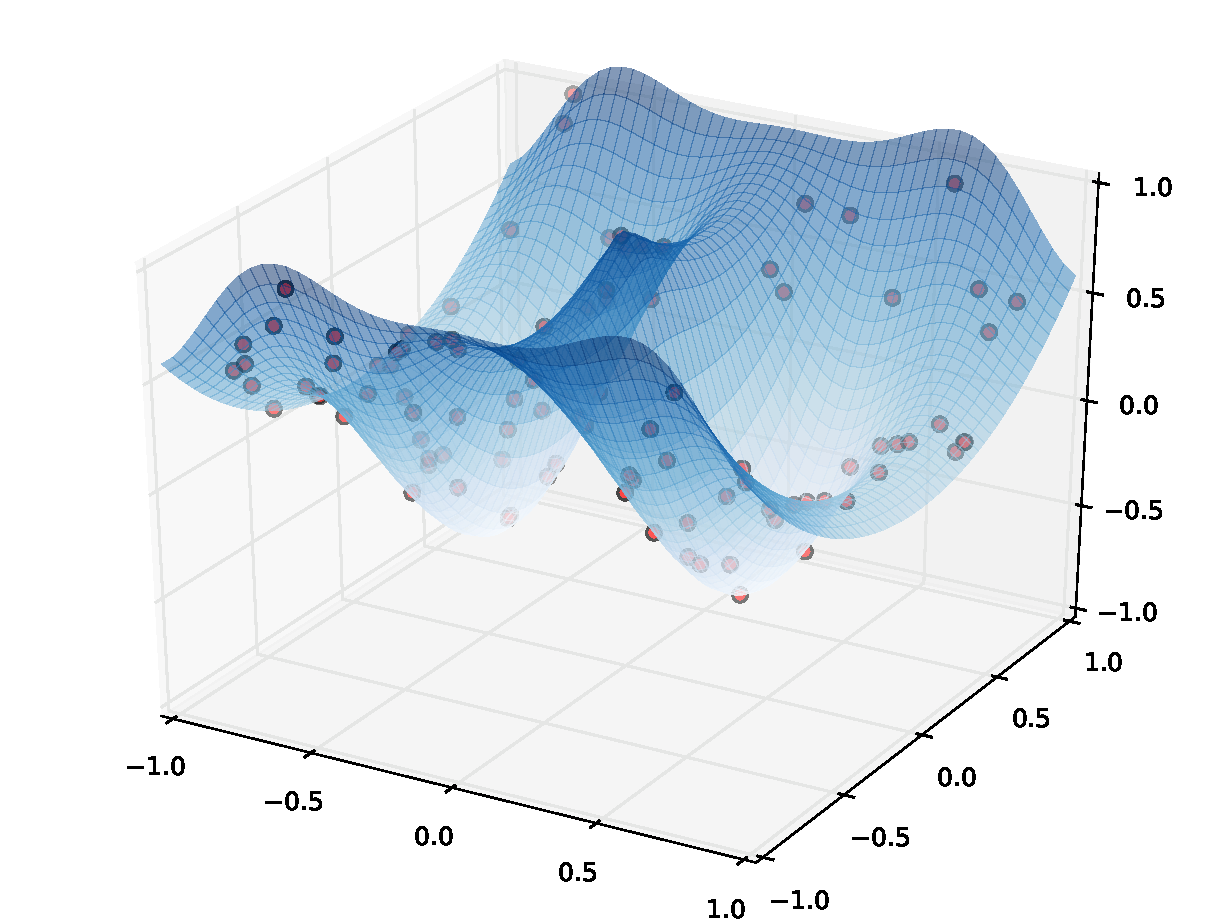
\includegraphics[width=\textwidth]{2DGaussianProcess1.pdf}
                \caption{Simulated elevation map with sampled points.}
                \label{fig:elevation}
        \end{subfigure}%
        ~ %add desired spacing between images, e. g. ~, \quad, \qquad etc. 
          %(or a blank line to force the subfigure onto a new line)
        \begin{subfigure}[b]{0.5\textwidth}
                \centering
                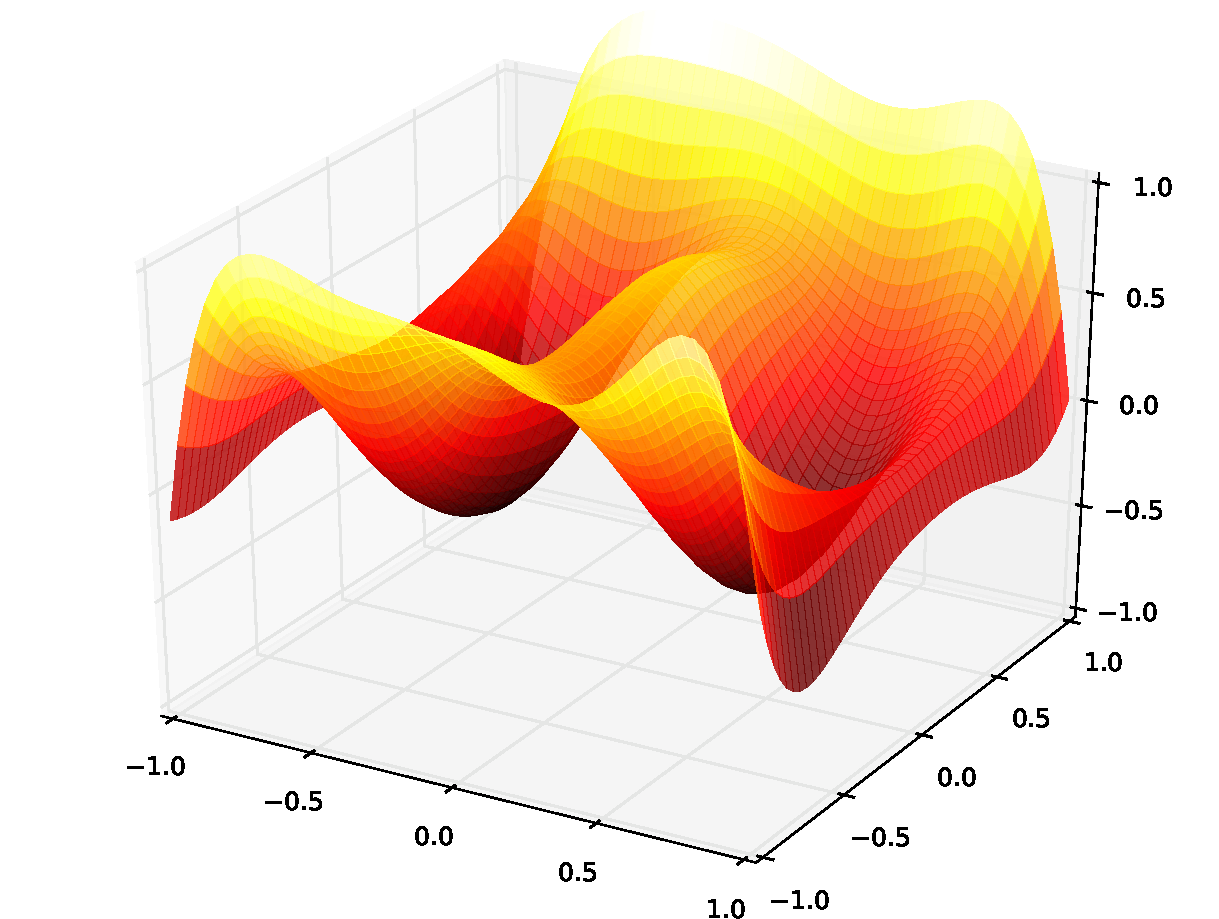
\includegraphics[width=\textwidth]{2DGaussianProcess2.pdf}
                \caption{Reconstructed mean surface from a grid of $X'$}
                \label{fig:mean}
        \end{subfigure}
        \caption{The left shows a real surface with samples drawn from it, representing $\mathbf{X}$. The right shows the mean construction using a grid of points, $\mathbf{X'}$}\label{fig:GP}
\end{figure}

\begin{figure}
\begin{center}
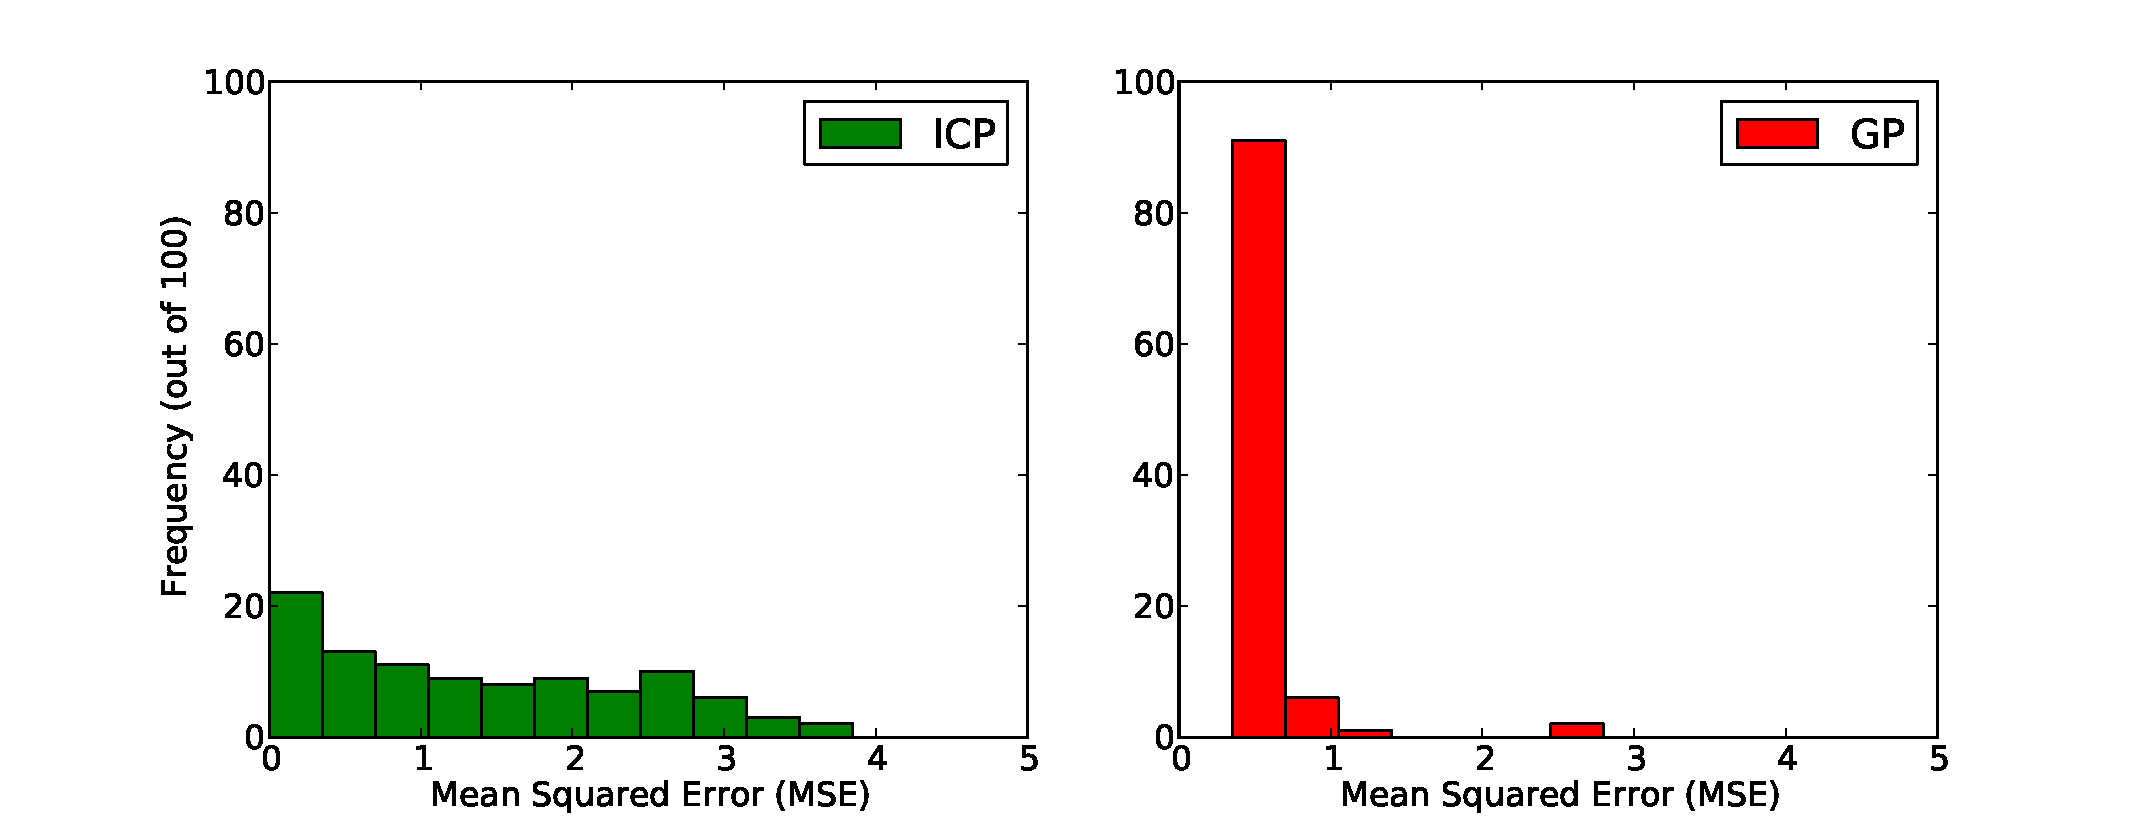
\includegraphics[width=5in]{goodnessoffit2.pdf}
\end{center}
\caption{Goodness of fit results for 100 random $T$.}
\label{figure:mse}
\end{figure}



\section{Experimental Setup}

For the following experiments, we generated simulated elevation data. An example elevation map can be seen in Figure \ref{fig:elevation}.


\section{Results}

ICP converges faster, but often to a poorer local minimum.

\section{Conclusion}
Gaussian Processes can represent and recover the transformation of a 3D scene. The convergence rate of Gaussian Processes outperforms ICP,
and the speed is not too much slower. The performance needs to be evaluated with real point cloud data, and subsampling of both the scene and the new points should be considered as a possible speedup. Real point cloud data might also warrant a different choice of kernel or further tuning of the kernel parameters. It is also important to try an experimental evaluation of the Newton's method-based optimization.
We noticed much better performance with small transformations, which motivated the constrained version of our problem. We did not discuss how to choose the constraints $\epsilon_1$ and $\epsilon_2$---if a real system was being built, these would be derived from the angular velocity, speed, and frame rate of the camera. 

\bibliographystyle{./IEEEtran}
% argument is your BibTeX string definitions and bibliography database(s)
\bibliography{./IEEEabrv,./full}

\section{Appendix}

\begin{figure}
\begin{center}
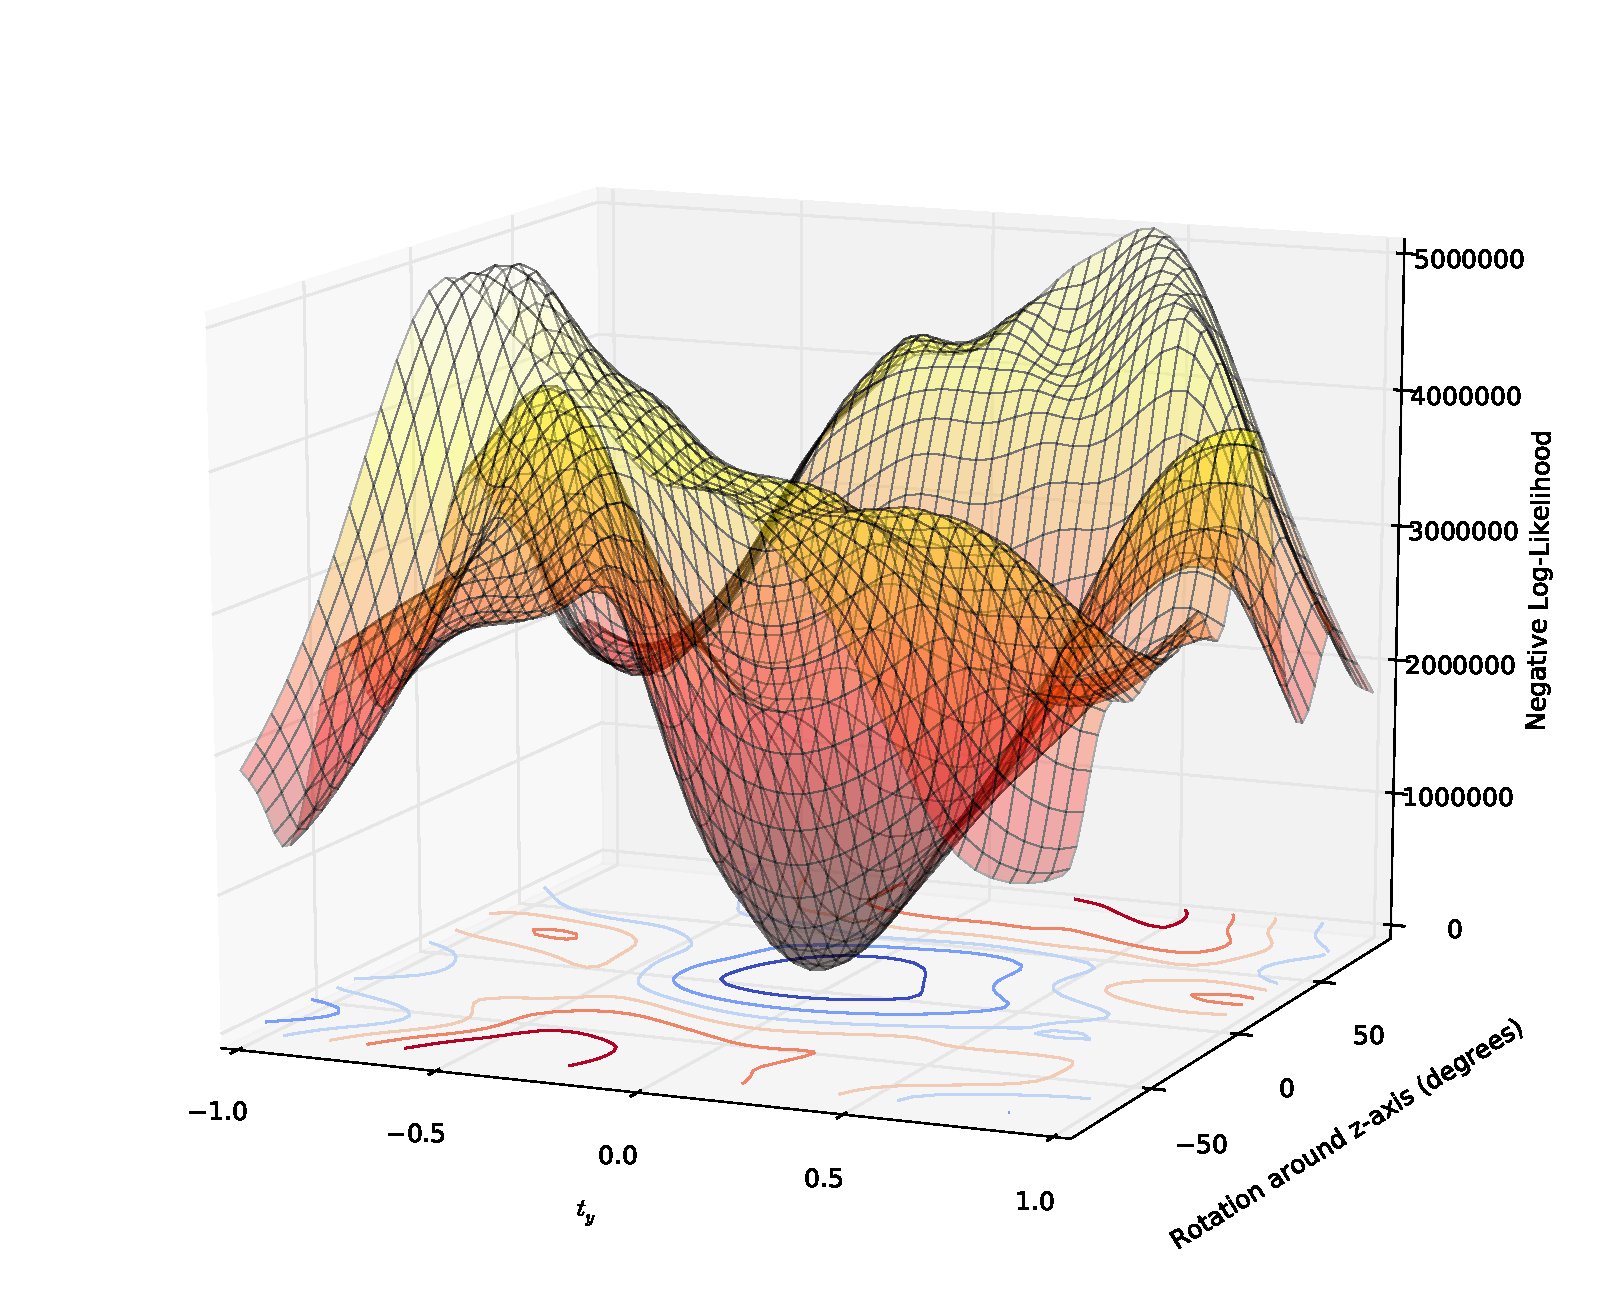
\includegraphics[width=6in]{LLmap3.pdf}
\end{center}
\caption{2-D Projection of the likelihood along $t_y$ and $\theta_z$}
\label{figure:likelihood}
\end{figure}
\end{document}